\section{Realizacja projektu}
Realizacja projektu Meetspace została podzielona na kilka etapów. Pierwszymi z nich było przygotowanie środowiska, zarejestrowanie domeny i zaprojektowanie modelu aplikacji. Następnie rozpoczęły się prace nad poszczególnymi funkcjonalnościami aplikacji, których etapy powstawania zostały udokumentowane w pliku \emph{CHANGELOG.md}


Poniżej zostały opisane wybrane funkcjonalności, działania i zagadnienia z zakresu back-ednu\footnote{działania aplikacji wykonywane po stronie serwera}, front-endu\footnote{działania aplikacji wykonywane po stronie przeglądarki intenetowej} i bezpieczeństwa aplikacji.
  \clearpage
  \subsection{Model bazy danych}
    Do przechowywania danych w aplikacji została wybrana baza SQlite, która w przyszłości zostanie zmieniona na MySQL. Baza zawiera cztery tabele:
    \begin{itemizeReduced}
      \item User - informacje o użytkowniku aplikacji
      \item Event - informacje związane z wydarzeniem
      \item Authentication - informacje pobrane z facebook api
      \item Subscriber - lista osób zapisanych do newslettera
    \end{itemizeReduced}

    \begin{figure}[h]
      \centering
        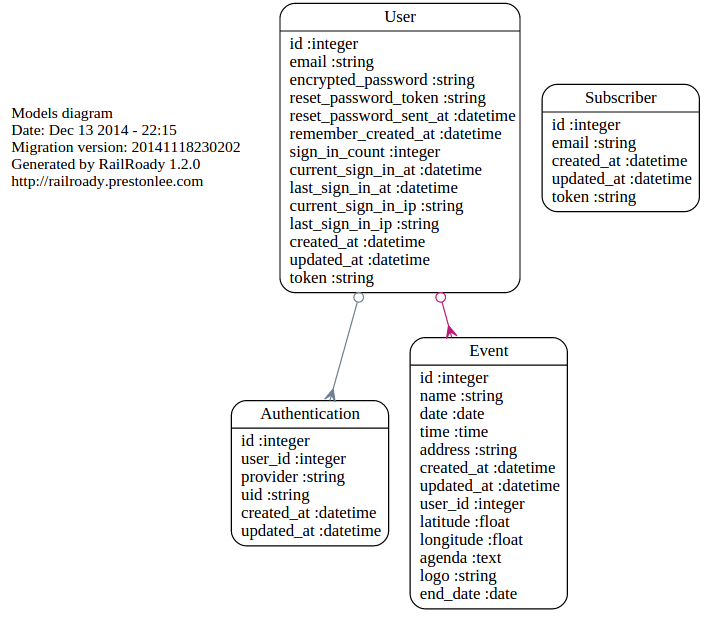
\includegraphics[scale=0.55]{images/dbm.png}
      \caption{Schemat bazy danych aplikacji Meetspace}
    \end{figure}

    Na rysunku nr \ref{fig:dbm} zamieściliśmy schemat bazy zapisany w pliku \texttt{schema.rb}, wygenerowany za pomocą mechanizmu migracji\footnote{Mechanizm wbudowany w Ruby on Rails pozwalający na modyfikowanie bazy danych za pomocą specjalnych plików, tzw. migracji opisujących poszczególne elementy bazy\cite{rails4_way}}.

\begin{code}
  \lstinputlisting[language = Ruby, basicstyle=\ttfamily\scriptsize, showstringspaces=false, breaklines=true, linerange={2-55, 57-57}]{../meetspace/db/schema.rb}
\end{code}


    % \subsection{Wyszukiwanie wydarzeń}
    % \subsection{Newsletter}

    \subsection{Przykładowe CSS i JS}
      W aplikacji zostały użyte takie technologie jak SASS\footnote{Więcej informacji w rozdziale \ref{other_technology}} i CoffeScript\footnote{Więcej informacji w rozdziale \ref{other_technology}}, które ułatwiły pracę nad wyglądem strony oraz jej funkcjonalnością po stronie przeglądarki internetowej.

      \subsubsection{CSS}
        Style CSS \emph{(Cascade Stylesheets)} stanowią o całej szacie graficznej aplikacji. Od nich zależy jak wygląda strona. Określają kolory, rozmiar czcionek, wielkości poszczególnych elementów czy nawet proste animacje. Bez tego strona wyglądałaby nieatrakcyjnie i byłaby zupełnie nie użyteczna.
        \begin{itemize}
          \item Flexbox\\
            To nowe rozwiązanie pozwalające uzyskać płynny layout\footnote{Dopasowyjący się do rozmiaru okna wygląd strony.}. Pomaga również wyśrodkować w pionie jeden element HTML względem drugiego. Dotychczas twórcy witryn internetowych musieli stosować różnego rodzaju sztuczki, żeby to osiągnać. Na dzień dziejszy\footnote{Dane z dnia 14.12.2014} flexbox jest wspierany przez większość czołowych przeglądarek\footnote{\url{http://caniuse.com/\#search=flexbox}}. \\
            Z tej technologii korzystaliśmy głównie do wyśrodkowania poszczególnych elementów wzgladem innych.

\begin{code}
	\lstinputlisting[linerange={14-18}, firstnumber=1]{../meetspace/app/assets/stylesheets/_variables.css.scss}
\end{code}\\

Fragment kodu powyżej to przykład oferowanej funkcjonalności preprocesora Sass. \emph{Mixin} to funkcja, która może być wielokrotnie wykorzystana na wielu selektorach CSS.

\begin{code}
	\lstinputlisting[linerange={38-40, 75-75}, firstnumber=1]{../meetspace/app/assets/stylesheets/welcome.css.scss}
\end{code}\\

\emph{@include flex(left)} rozszerzy klasę \emph{search} o właściwości wymienione w pierwszym fragmencie kodu.

Rezultat zastosowania mechanizmu flexbox:\\
\begin{figure}[h]
	\centering
  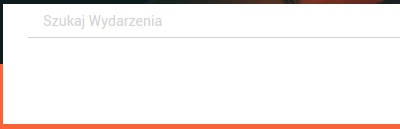
\includegraphics[scale=0.8]{images/flex_before.png}
  \caption{Bez flexbox.}
\end{figure}

\begin{figure}[h]
	\centering
  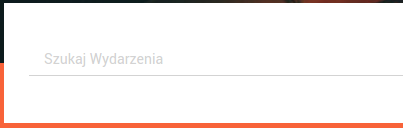
\includegraphics[scale=0.8]{images/flex_after.png}
  \caption{Z wykorzystaniem flexbox.}
\end{figure}


          \item Placeholder\\
            Placeholder to napis wyświetlany w ramce do wpisywania tekstu przez użytkownika. Służy do informowania o roli danego pola. Domyślnym kolorem czcionki jest szary ale nam zależało, żeby cały wygląd współgrał ze sobą. Dlatego chcieliśmy aby kolor placeholder'a był nieco jaśniejszy. Niestety nie da się tego osiągnąć nadając tagowi \emph{input} jakąś klasę i jej ustawiając kolor. Jedyny sposób to wykorzystanie predefiniowanego selektora, odpowiedzialnego za wygląd placeholder'a.

            \begin{code}
              \lstinputlisting[linerange={95-108}, firstnumber=1]{../meetspace/app/assets/stylesheets/layout.css.scss}
            \end{code}\\

            Wartość \emph{\$placeholder} to zmienna Sass przechowująca kolor. Dzięki jej zastosowaniu, w przypadku gdybyśmy chcieli zmienić wartość koloru na inną, nie będziemy musieli tego robić w kilku miejscach, tylko w jednym.

          \item Zapytania medialne \emph{(Media Queries)}\\
            W trakcie tworzenia witryny, która ma dopasowywać się do wielkości ekranu urządzenia, kluczową rolę odgrywają zapytania medialne. W trakcie ładowania pliku css, sprawdzają wielkość, rodzaj ekranu i stosują style zadeklarowane dla konkretnych rozdzielczości. Dzięki temu można określić na przykład, aby dla urządzeń o szerokości ekranu większej niż 600 pixeli tło strony było inne niż dla węższych ekranów.
            Poniżej zastosowane przez nas zapytania medialne dla urządzeń o maksymalnej szerokości 767 pixeli.
            \begin{code}
              \lstinputlisting[linerange={3}]{../meetspace/app/assets/stylesheets/media_queries.css.scss}
            \end{code}\\
        \end{itemize}
    % \subsection{Bezpieczeństwo}
    %   \begin{itemize}
    %     \item current\_user
    %     \item boot
    %     \item autoryzacja api
    %     \item walidacje
    %     \item SQL injection
    %     \item XSS
    %   \end{itemize}
    % \subsection{Przegląd widoków aplikacji}
    %   \begin{itemize}
    %     \item responsywnść, czli o gridach
    %     \item html 5, a co jak nie działą :P?
    %   \end{itemize}

